\documentclass[11pt,a4paper]{article}
\usepackage{graphicx}
\usepackage{float}
\graphicspath{ {../scientific-experimentation-evaluation/} }
\usepackage{color}
\usepackage{listings}
\usepackage{hyperref}
\usepackage{amsmath}

\begin{document}
	\title{\textbf{Scientific Experimentation and Evaluation \\ Assignment 4}}
	\author{Aaqib Parvez Mohammed \\ Chetan Sidnal\\ Mihir Patil \\ Sushma devaramani}
	\date{\today}
	\maketitle
	\newpage
	\tableofcontents
	\newpage
	\listoffigures
	\newpage
	\section{Experiment 1: Manual Motion Observation}
	\textbf{Aim:} Manually measure the observable pose variation for three different constant velocity motions(Straight line, an arc to the left and an arc to the right) of LEGO NXT differential drive robot.
	
	\subsection{\textbf{Setup}}
	\begin{itemize}
		\item The measurement system for the experiment includes a white sheet, a LEGO NXT differential drive robot, two pencils and a scale.
		\item The \textbf{device under test(DUT)} is the LEGO NXT differential drive robot.
		\item Clamp the sheet on a flat surface.
		\item Construct a robot equipped with two pencils in the front, such that the start and end positions can be marked. This constitutes the measurement facility.
		\item Install \textit{Lejos} OS on the robot.
		\item Program the robot for it to run in three different constant velocity motions.
	\end{itemize}
	
	\begin{figure}[H]
		\centering
		\centering
		\includegraphics[width=0.8\linewidth]{1}
		\caption{Side view}
		\label{fig:side}
	\end{figure}
	
	\begin{figure}[H]
		\centering
		\centering
		\includegraphics[width=0.8\linewidth]{isometric}
		\caption{Isometric view}
		\label{fig:iso}
	\end{figure}
	
	\begin{figure}[H]
		\centering
		\centering
		\includegraphics[width=0.8\linewidth]{Top}
		\caption{Top view}
		\label{fig:top}
	\end{figure}
	
	\begin{figure}[H]
		\centering
		\centering
		\includegraphics[width=0.8\linewidth]{front}
		\caption{front view}
		\label{fig:front}
	\end{figure}
	
	\newpage
	\subsection{\textbf{Procedure}}
	\begin{itemize}
		\item The experimental setup is prepared.
		\item The starting position of the robot is marked with the help of the points drawn by the pencils.
		\item The center of the line joining the two points is recorded which will be the starting position of the robot.
		\item The robot is programmed to run in a straight line forward motion at a constant speed.
		\item Once the robot stops, the center of the line joining the last points drawn by the pencils will be the stop position.
		\item The \textbf{Measurand} i.e., the relative coordinates of the robot are measured by the difference in the coordinates of the starting position and the stopping position.
		\item \textbf{Measurement System:} Our measurement system consists of robot placed on a cardboard sheet. Two pencils are attached in the front to mark the position. As the robot is moved, the path is traced on the sheet. After reaching the end position, the final pose is marked. The variation in the path is observed and the error in pose is measured.
		\item The \textbf{Measurement result} i.e., the pose variation is obtained by finding the difference between the observed values and their mean.
		\item Repeat the above experiment with a program to run the robot with constant angular and translational velocities for a fixed time period, such that it describes an arc to the left.
		\item Repeat the above experiment with a program to run the robot with constant angular and translational velocities for a fixed time period, such that it describes an arc to the right.
	\end{itemize}
	
	\subsection{\textbf{Expected problems}}
	\begin{itemize}
		\item Parallax error.
		\item Positional errors.
		\item There might be slipping of wheels.
		\item The tip of the pencils might break during the motion of the robot.
		\item The pencils will have to be sharpened as the nibs might get blunt due to continuous drawing of lines which might result in measurement errors.
	\end{itemize}
	
	\subsection{\textbf{Expected performance}}
	\begin{itemize}
		\item The Rotation sensor measures the motor rotations with the accuracy of +/- one degree for one rotation(360 degree). Hence the accuracy in distance traveled for one rotation will be +/- 0.05 cm. 
		\item Reference: LEGO NXT: Features \& Limitations.
		\item Assuming experiment distance = 70.4 cm.
		\item Expected accuracy is $ \pm 2$ and expected precision is 70.4$ \pm 0.2$cm.
	\end{itemize}
	
	\subsubsection{Reasons}
	\begin{itemize}
		\item The slippage of the wheels may cause poor accuracy and precision.
		\item The internal errors from the DUT may cause poor accuracy but the precision won't be affected significantly, since the DUT won't be changed while doing the measurement.
	\end{itemize}
	
	\subsection{Execution of the experiment:}
	\begin{itemize}
		\item The starting position of the robot was marked using two pencils which were placed on either side of the robot.
		\item The same points were used as the starting points while repeating the experiment.
		\item The position of the back wheel was also kept constant by drawing a line and using the same line as reference for future run of experiments.
		\item The position of the back wheel impacted the outcome of the experiment as a small deviation from the reference line would result in a considerable deviation of the outcome.
		
		\item The theta values were calculated by drawing a perpendicular to the line joining the two observed end points and calculating the angle using the formula $tan^{-1}(\frac{y}{x})$. As shown in the below figure.
		\begin{figure}[H]
			\centering	
			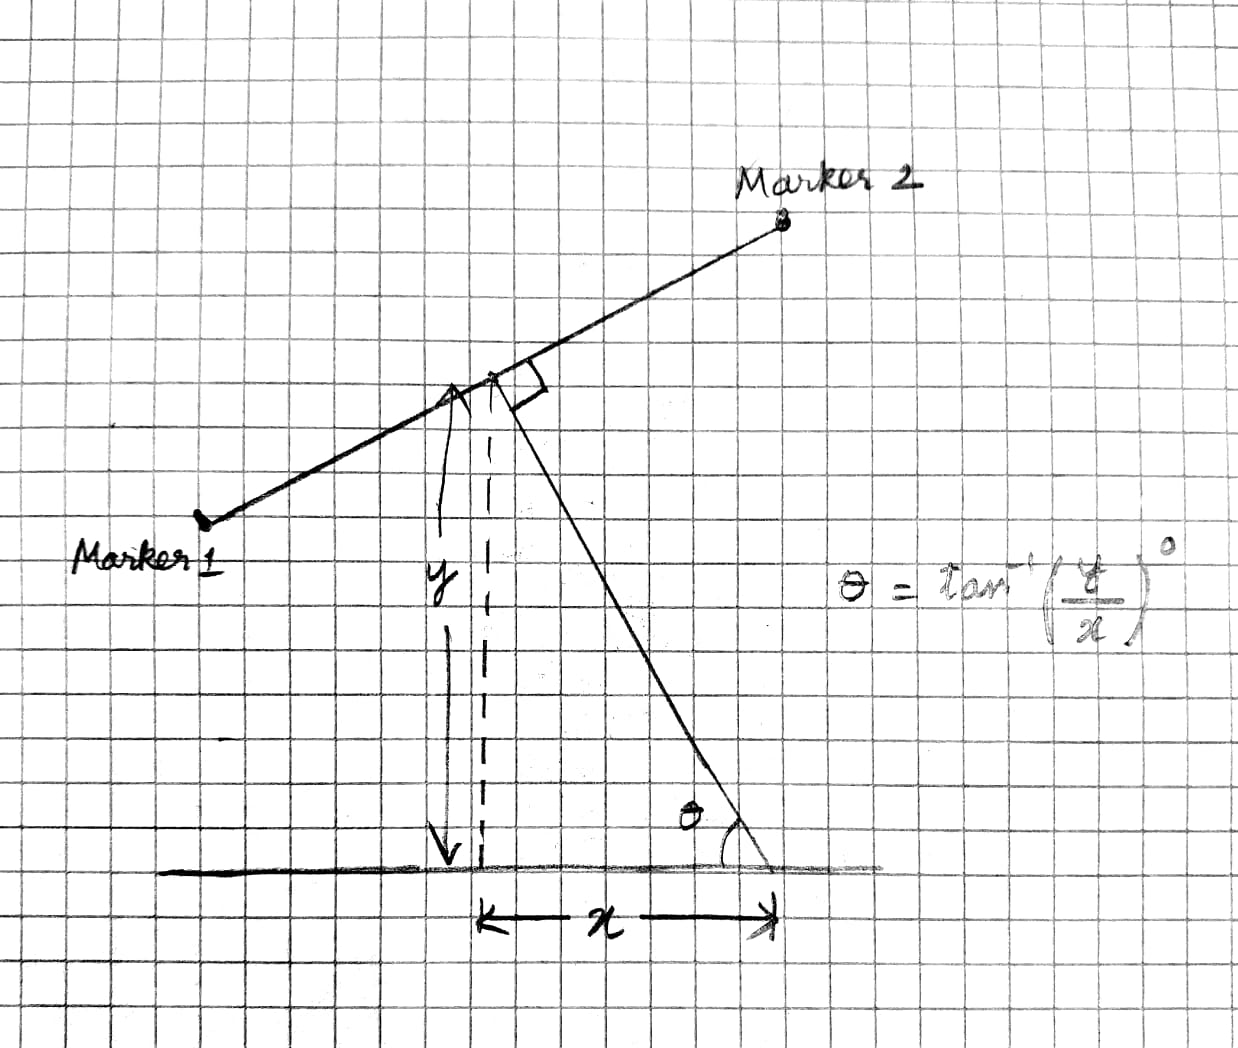
\includegraphics[width=1.2\linewidth]{theta_calc.jpeg}
			\label{fig:theta_calc}
			\caption{Finding out $\theta$ for robot orientation}
		\end{figure}
		\item Lego NXT 2.0 software was used to program the robot with the following parameters.\\
		No. of rotations = 4\\ 
		Power = 40
		\item \textcolor{blue}{The battery voltage before the experiment = 8.2V. \\ The battery voltage after the experimenter = 4.2V.}
		\item The observed data has been recorded in the ".csv" format.
		\item There was no pre-processing of data required as no outliers were detected.
		\item Graph has been plotted for all three motions. \\
		Note : All x,y measurements are in centimeters (cm)
		\subsubsection{Straight}
		\begin{figure}[H]
			\centering	
			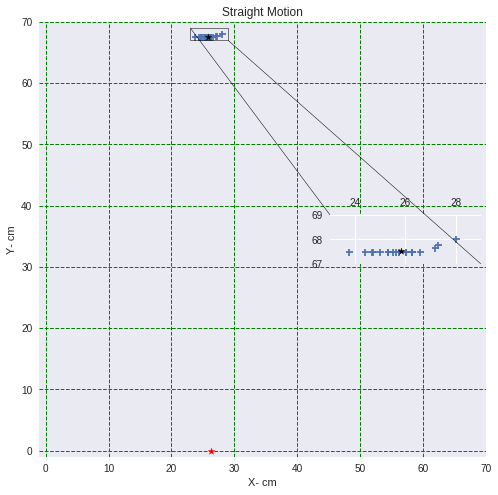
\includegraphics[width=1.2\linewidth]{Straight}
			\label{fig:straight}
			\caption{20 iteration of moving straight}
		\end{figure}
		
		\newpage
		\textbf{Fitting the distribution for the obtained data: \\ (X, Y) points for straight line}
		\begin{figure}[H]
			\centering	
			\includegraphics[width=0.8\linewidth]{straightG}
			\label{fig:straightG}
			\caption{Density plot of (X,Y) for straight line motion}
		\end{figure}
		
		In the above graph, it can be observed that 'X' points fit a gaussian distribution, whereas 'Y' points does not fit any distribution, since they are mostly precise and accurate.
		%   \begin{figure}[H]
		% 	\centering	
		% 		\includegraphics[width=1.0\linewidth]{bplot_straight}
		% 		\label{fig:sub1}
		% 	\caption{\color{blue}Box plot for (X, Y) points in straight line}
		%   \end{figure}
		\begin{itemize}
			\item $ Range (x,y) =([23.8-28.1],[67.5-68.1]) $
			\item $ Mean (x, y) = 25.8,67.5$
			\item $ \sigma (x, y)= 1.1, 0.1 $
			\item $ Precision (x, y)= 25.8 \pm 1.1, 67.5 \pm 0.1  $
			\item $ Accuracy (x,y) = x \pm0.9  , y \pm0.1 $  
		\end{itemize}
		
		\subsubsection{Right}
		\begin{figure}[H]
			\centering	
			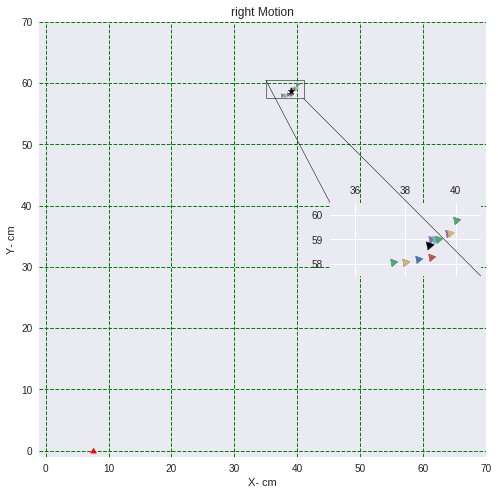
\includegraphics[width=1.2\linewidth]{right_cm}
			\label{fig:right}
			\caption{20 observations of right arc motion}
		\end{figure}
		
		\begin{figure}[H]
			\centering	
			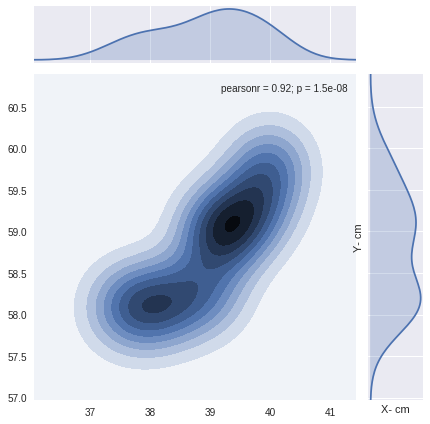
\includegraphics[width=0.8\linewidth]{rightG}
			\label{fig:sub1}
			\caption{Density plot of (X, Y) points for right arc motion}
		\end{figure}
		
		In the above plot it can be observed that the distribution of X and Y positions for right arc motion is gaussian.
		%   \begin{figure}[H]
		% 	\centering	
		% 		\includegraphics[width=1.0\linewidth]{dist_plot}
		% 		\label{fig:sub1}
		% 	\caption{\color{blue}20 iteration distribution plot}
		%   \end{figure}
		
		\begin{itemize}
				\item $ Range (x,y) =([37.5-40.0],[58.0-59.8])  $
				\item $ Mean (x, y) = 38.9,58.8$
				\item $ Precision (x, y)= 38.9 \pm 0.8, 58.8 \pm 0.6 $
				\item $ Accuracy (x,y) = x \pm0.5 , y \pm0.5  $ 
				\item $ \sigma (x, y)= 0.8, 0.6 $
				\item $ Mean(\theta) = 40.6 degree$
				\item $ Accuracy (\theta)= \theta \pm5  deg $
				\item $ \sigma = 1.1 deg$
				\item $ range (\theta) = 38.8 - 43.3 $
			\end{itemize}
			
			\subsubsection{Left}
			\begin{figure}[H]
				\centering	
				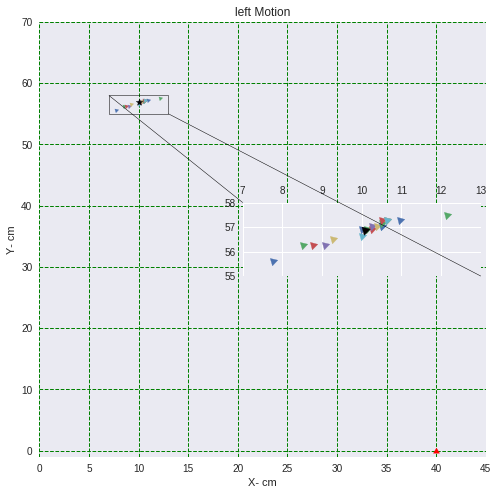
\includegraphics[width=1.2\linewidth]{left_cm}
				\label{fig:sub1}
				\caption{20 iteration of moving left}
			\end{figure}
			
			\begin{figure}[H]
				\centering	
				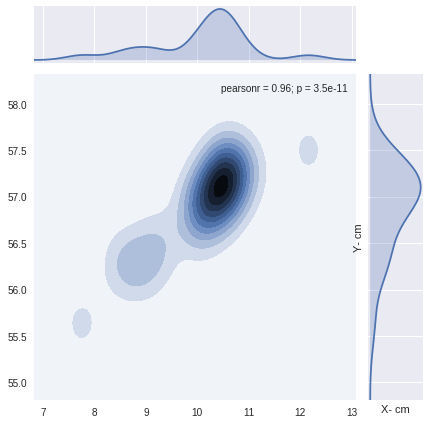
\includegraphics[width=1.0\linewidth]{leftG}
				\label{fig:sub1}
				\caption{Density plot of (X, Y) for moving left}
			\end{figure}
			
			In the above figure it can be observed that the (X, Y) points obtained for left arc motion fit a gaussian distribution.
			%   \begin{figure}[H]
			% 	\centering	
			% 		\includegraphics[width=1.0\linewidth]{bplot_left}
			% 		\label{fig:sub1}
			% 	\caption{\color{blue}Box plot for 20 iterations of left arc motion}
			%   \end{figure}
			\begin{itemize}
					\item $ Range (x,y) =([7.8-12.2],[55.6-57.5])  $
					\item $ Mean (x, y) = 10.1,56.9$
					\item $ Precision (x, y)= 10.1 \pm 2.0, 56.9 \pm 1.5 $
					\item $ Accuracy (x,y) = x \pm0.5 , y \pm0.5  $ 
					\item $ \sigma (x, y)= 1.0, 0.5 $
					\item $ Mean(\theta) = 45.7 degree$
					\item $ Accuracy (\theta)= \theta 7\pm  deg $
					\item $ \sigma = 1.3 deg$
					\item $ range (\theta) = 43.2 - 48.3 $
				\end{itemize}
			\end{itemize}
			
			% \subsection{Straight Motion}
			% \begin{table}
			% \centering
			% \pgfplotstabletypeset[dec sep align,
			%    fixed zerofill,
			%    precision=4,
			%    col sep=space]{leftT.csv}
			% \end{table}
			
			% \subsection{Right Motion}
			
			% \subsection{Left Motion}
			
			\textbf{Boxplots}
			\begin{figure}[H]
				\centering
				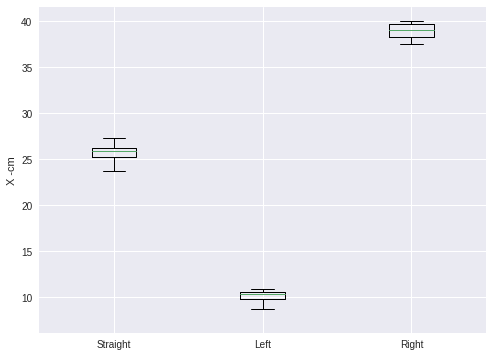
\includegraphics[width=1.0\linewidth]{boxplot-x}
				\label{fig:box-x}
				\caption{Box plot of X-values for straight line motion, left and right turn}
			\end{figure}
			
			\begin{figure}[H]
				\centering	
				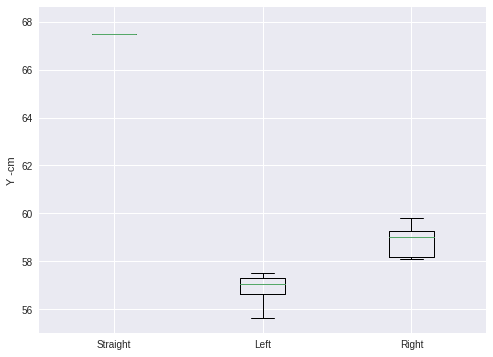
\includegraphics[width=1.0\linewidth]{boxplot-y}
				\label{fig:box-y}
				\caption{Box plot of Y-values for straight line motion, left and right turn}
			\end{figure}
			
			\begin{itemize}
				\item 2.3 The chi-square test indicates that the observed data is a normal distribution.
\begin{lstlisting}[language=Python]
In [9]: ks , p = stats.normaltest(straight_xy)
alpha = 1e-3
# null hypothesis: x comes from normal distribution
if p.all() < alpha: 
print("The null hypothesis can be rejected")
else:
print("The null hypothesis cannot be rejected")

[Out]: The null hypothesis cannot be rejected

In [10]: ks , p = stats.normaltest(right_xy)
alpha = 1e-3
if p.all() < alpha: 
print("The null hypothesis can be rejected")
else:
print("The null hypothesis cannot be rejected")
[Out]: The null hypothesis cannot be rejected

In [11]: ks , p = stats.normaltest(left_xy)
alpha = 1e-3
if p.all() < alpha: 
print("The null hypothesis can be rejected")
else:
print("The null hypothesis cannot be rejected")
[Out]: The null hypothesis cannot be rejected
\end{lstlisting}
				
				\item Deliverable 2.2: The functions used for plotting are from the seaborn library and use a kernel density method to obtain a 2-D density plot of the x and y coordinates. 
				\item Deliverable 2.5:\\
				
				\textbf{Straight:}  In the case of straight line motion the readings obtained for Y coordinates appear to be both precise and accurate, whereas the X coordinates appear to be precise but not very accurate. \\
				
				\textbf{Right:} The readings obtained for Y coordinates appear to be both highly precise and accurate, whereas the X coordinates appear to be precise but not very accurate. \\
				
				\textbf{Left:} The readings obtained for X coordinates appear to have low precision and accuracy, whereas the Y coordinates appear to be precise with a low accuracy.
				\textcolor{blue}{\item \textbf{Comparison of Actual performance with expected:} \begin{itemize} \item The expected distance to be traveled was 70.4 cm.
						\item The mean actual distance travelled was calculated by applying distance formula on initial and end points, which is equal to 67.5 cm.
						\item Estimated error = 2 cm
						\item Actual error = 2.9 cm
						\item The difference in the actual and expected error can be due to systematic or/and random errors.
					\end{itemize}}
				\end{itemize} 
				\newpage
				\section{Calibrating an Optical Tracking System}
				\subsection{Setup for camera calibration }
				\begin{itemize}
					\item The camera calibration process is done on a checkerboard (calibration tool).
					\item The \textit{MATLAB support package for USB webcam} for camera calibration is installed.
					\item The camera calibration toolbox for MATLAB is installed.
					\item The webcam (Microsoft Lifecam) is connected to the laptop and the connectivity is checked by running \textit{webcam list} command in MATLAB, which shows the list of all webcams connected to PC.
					\item The webcam is mounted on a static paper punch, while capturing the images.
					\item The Auto-focus is turned \textit{off} by running the following command in MATLAB,
					\begin{lstlisting}
cam.FocalMode = manual
					\end{lstlisting}
					\item The images of checkerboard are captured from different perspectives (different position and orientation in the camera's field of view). A total of 20 images are captured and saved for the calibration process.
				\end{itemize}
				
				\subsection{Estimation of number of images}
				\begin{itemize}
					\item Since the object in the world is 3-dimensional and the captured images are 2D (co-planar), we loose one dimension. In order to regain the actual dimensionality during the calibration, various number of images are captured in different positions and orientations. 
					\item As a rule of thumb, 20-40 images is quite enough for the process. For our calibration we have captured 20 images in different position and orientations. 
					\item The idea behind the capturing enough images is to cover the field of view, and to have a good distribution of 3D orientations of the board. 
				\end{itemize}
				
				
				\subsection{Description of the camera parameters}
				After the calibration, the list of parameters obtained are of two types.
				\begin{itemize}
					\item \textbf{Intrinsic parameters}
					\begin{itemize}
						\item \textbf{Focal length:} Distance between the lens and the image sensor when the object is in focus, usually stated in millimeters. The focal length in pixels is stored in the 2x1 vector $fc$. 
						\item \textbf{Principal point:} A point at the intersection of the optical axis and the image plane. The principal point coordinates are stored in the 2x1 vector $cc$.
						\item \textbf{Skew coefficient:} Defines the angle between x and y pixels axes and is stored in $alpha_c$
						\item \textbf{Radial Distortions:} Symmetric distortion caused by the lens due to imperfections in curvature when the lens was ground.
					\end{itemize}
					\item \textbf{Extrinsic parameters}
					\begin{itemize}
						\item \textbf{Rotational Vectors:} Vector describing the rotation of camera plane with respect to the world frame.
						\item \textbf{Translational vectors:} Vector describing the translation of camera plane with respect to the world frame.
					\end{itemize}
				\end{itemize}
				
				\subsection{Possible problems or error sources that can disturb the calibration process}
				\begin{itemize}
					\item If the naming conventions of the images are different, then the calibration process gives error.
					\item The computer running the calibration toolbox must have enough RAM(128 MB or less). If this condition is not met, then it gives \textit{OUT OF MEMORY} error.
					\item Enough number of images must be provided to get better calibration results.
					\item The images captured with same orientations will not provide enough inputs for the toolbox to calibrate efficiently.
				\end{itemize}
				
				\subsection{Image poses used for calibration}
				
				\begin{figure}[H]
					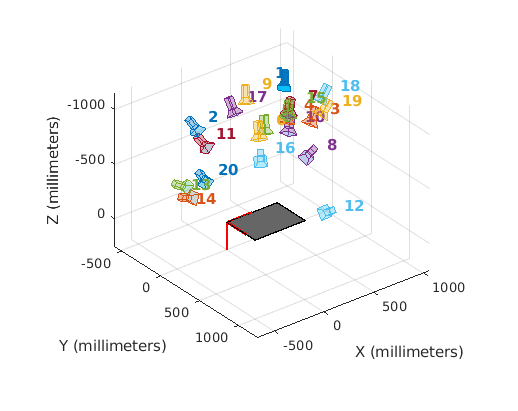
\includegraphics[scale=0.7]{pattern_centric_view.png}
					\caption{Pattern centric view}
				\end{figure}
				
				\begin{figure}[H]
					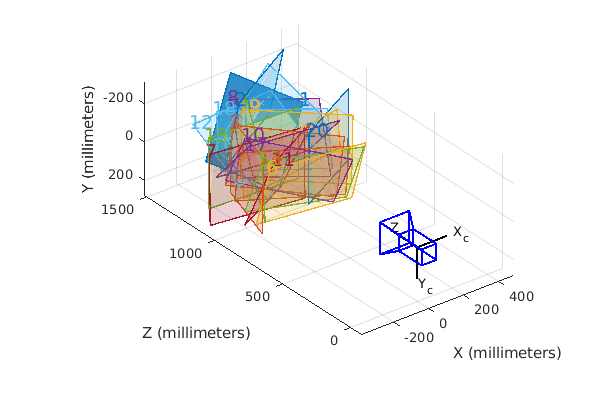
\includegraphics[scale=0.7]{camera_centric_view.png}
					\caption{Camera centric view}
				\end{figure}
				The image poses can be approximated using the figures presented above which are obtained using the MATLAB camera calibration toolbox. However the exact values of each of these images poses is not possible to obtain due to a lack of a suitable measuring metric.
				\subsection{Camera parameters obtained from calibration}
				\[ 
				Intrinsic Matrix =
				\begin{bmatrix}
				648.7381 & 0 & 0 \\
				-0.5603 & 648.5722 & 0 \\
				417.6238 & 285.6146 & 1 \\
				\end{bmatrix}
				\]
				\[ 
				Focal Length =
				\begin{bmatrix}
				648.7381 & 648.5722
				\end{bmatrix}
				\]
				\[ 
				Principal point =
				\begin{bmatrix}
				417.6238 & 285.6146
				\end{bmatrix}
				\]
				\[ 
				Skew = -0.5603
				\]
				\[
				Radial distortion = 
				\begin{bmatrix}
				-0.0183 & 0.1165
				\end{bmatrix}
				\]
				\[ 
				Tangential Distortion = 
				\begin{bmatrix}
				-0.0016 & 9.2118e-04
				\end{bmatrix}
				\]
				\[ 
				Mean projection error = 0.1516
				\]
				\subsection{Estimation errors}
				\subsubsection{Intrinsic errors}
				\[
				Skew error = 0.1173
				\]
				\[
				Focal length error = 
				\begin{bmatrix}
				0.3475 & 0.3245
				\end{bmatrix}
				\]
				\[
				Principal point error = 
				\begin{bmatrix}
				0.6292 & 0.5130
				\end{bmatrix}
				\]
				\[
				Radial distortion error = 
				\begin{bmatrix}
				0.0028 & 0.0134
				\end{bmatrix}
				\]
				\[
				Tangential distortion error
				\begin{bmatrix}
				2.8109e-04 & 3.5275e-04
				\end{bmatrix}
				\]
				\subsubsection{Extrinsic errors}
				They are available in the \textit{estimationerrors.mat} file
				
				
				\subsection{Arguments for which camera model best fits} 
				If the lens distortions are really too severe (for fish-eye lenses for example), the simple guiding tool based on a single distortion coefficient kc may not be sufficient to provide good enough initial guesses for the corner locations. then corner extraction has to be done manually.
				
				\newpage
				\section{Appendix}
				\subsection{Softwares used}
				\begin{itemize}
					\item Python 2.7
					\item Jupyter Notebook
				\end{itemize}
				
				\subsection{Packages used}
				\begin{itemize}
					\item Matplotlib
					\item Numpy
					\item Scipy
					\item Seaborn
					\item Pylab
				\end{itemize}
				
				\subsection{Tools used}
				\begin{itemize}
					\item Onscreen ruler is used to mark scale on the sheet (metrics in inches)
					\item \url{https://www.piliapp.com/actual-size/inch-ruler/}
					\begin{figure}[H]
						\centering	
						\includegraphics[width=0.4\linewidth]{screenshot}
						\label{fig:sub1}
						\caption{Online ruler}
					\end{figure}
					
					\begin{figure}[H]
						\centering	
						\includegraphics[width=0.7\linewidth]{measure}
						\label{fig:sub1}
						\caption{Marking scale on the sheet using onscreen ruler}
					\end{figure}
					
				\end{itemize}
			\end{document}
